\section{HTTT Proxy}

\begin{frame}{Proxy}{Stellvertreter}
  \begin{center}
 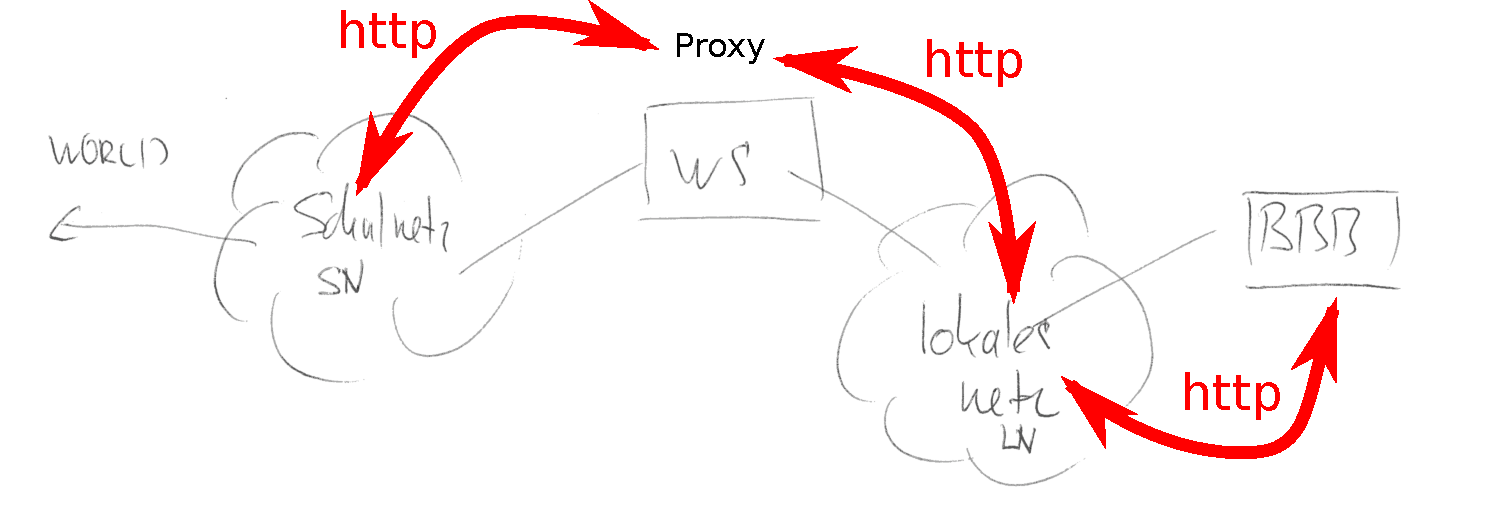
\includegraphics[width=0.875\textwidth]{proxy.pdf}
 \end{center}
 \vspace{-1.5cm}
 \begin{itemize}
  \item Server auf \host
  \item reicht die \cod{http} {\em requests/responses} weiter
 \end{itemize}
 \remark{funltioniert nur f�r \cod{http}}
\end{frame}

\begin{frame}{Test mit \cod{curl}}{\url{curl.haxx.se/}}
  \begin{itemize}
   \item \cod{curl address}
   \begin{itemize}
    \item \cod{curl fhnw.ch}
    \item \cod{curl -v address} \cod{-v}: verbose
   \end{itemize}
  \end{itemize}
\end{frame}

\begin{frame}{Proxy Server}{drei Vorschl�ge}
 \begin{itemize}
  \item \cod{tinyproxy}
  \vspace{-5mm}
  \begin{quote}
  lightweight http(s) proxy daemon
  \end{quote}
  \begin{itemize}
   \item {\scriptsize\url{tinyproxy.github.io}}
  \end{itemize}
  \item \cod{polipo}
   \vspace{-5mm}
   \begin{quote} 
   is a lightweight caching and forwarding web proxy server
   \end{quote}
%   \vspace{-5mm}
   \begin{itemize}
    \item {\scriptsize\url{www.pps.univ-paris-diderot.fr/~jch/software/polipo/}}
   \end{itemize}
  \item \cod{squid}
   \vspace{-5mm}
   \begin{quote} 
   is a caching proxy for the Web supporting
   \end{quote}
   \begin{itemize}
     \item {\scriptsize\url[http]{www.squid-cache.org/}}
   \end{itemize}
 \end{itemize}
\end{frame}


\begin{frame}{\cod{tinyproxy}}{direkter Aufruf}
 \begin{description}[\target]
  \item[\host] Skript Server
  \begin{itemize}
   \item \cod{./tools/tinyproxy.sh}
  \end{itemize}
  \item[\target] Client
  \begin{itemize}
   \item \cod{curl --proxy http://192.168.7.1:8888  \textbackslash\\ www.google.ch}
  \end{itemize}
 \end{description}
 \remark{Wie steht es mit \cod{https}}
\end{frame}

\begin{frame}{\target}{\cod{apt-get}}
 \begin{itemize}
  \item Konfiguration \targetS
  \begin{itemize}
   \item File \cod{/etc/apt/apt.conf.d/05proxy}
   \begin{itemize}
    \item \cod{Acquire::http::proxy "{}http://192.168.7.1:8888"{};}
   \end{itemize}
    \item Wie editieren:
    \begin{itemize}
     \item Auf dem \targetS mit \cod{vi}
     \item per \cod{sshfs} vom \host aus
    \end{itemize}
  \end{itemize}
  \item Test
  \begin{itemize}
   \item \cod{apt-get update}
   \item \cod{apt-get install sshfs}
  \end{itemize}
 \end{itemize}
\end{frame}
